%
% ---------------------------------------------------------------
% Copyright (C) 2012-2018 Gang Li
% ---------------------------------------------------------------
%
% This work is the default powerdot-tuliplab style test file and may be
% distributed and/or modified under the conditions of the LaTeX Project Public
% License, either version 1.3 of this license or (at your option) any later
% version. The latest version of this license is in
% http://www.latex-project.org/lppl.txt and version 1.3 or later is part of all
% distributions of LaTeX version 2003/12/01 or later.
%
% This work has the LPPL maintenance status "maintained".
%
% This Current Maintainer of this work is Gang Li.
%
%

\documentclass[
 size=14pt,
 paper=smartboard,  %a4paper, smartboard, screen
 mode=present, 		%present, handout, print
 display=slides, 	% slidesnotes, notes, slides
 style=tuliplab,  	% TULIP Lab style
 pauseslide,
 fleqn,leqno]{powerdot}


%我自己增加的两端对其用
\usepackage{ragged2e}
\renewcommand{\raggedright}{\leftskip=0pt \rightskip=0pt plus 0cm}


\usepackage{cancel}
\usepackage{caption}
\usepackage{stackengine}
\usepackage{smartdiagram}
\usepackage{attrib}
\usepackage{amssymb}
\usepackage{amsmath} 
\usepackage{amsthm} 
\usepackage{mathtools}
\usepackage{rotating}
\usepackage{graphicx}
\usepackage{boxedminipage}
\usepackage{rotate}
\usepackage{calc}
\usepackage[absolute]{textpos}
\usepackage{psfrag,overpic}
\usepackage{fouriernc}
\usepackage{pstricks,pst-3d,pst-grad,pstricks-add,pst-text,pst-node,pst-tree}
\usepackage{moreverb,epsfig,subfigure}
\usepackage{color}
\usepackage{booktabs}
\usepackage{etex}
\usepackage{breqn}
\usepackage{multirow}
\usepackage{natbib}
\usepackage{bibentry}
\usepackage{gitinfo2}
\usepackage{siunitx}
\usepackage{nicefrac}
%\usepackage{geometry}
%\geometry{verbose,letterpaper}
\usepackage{media9}
\usepackage{animate}
%\usepackage{movie15}
\usepackage{auto-pst-pdf}

%\usepackage{breakurl}
\usepackage{fontawesome}
\usepackage{xcolor}
\usepackage{multicol}



\usepackage{verbatim}
\usepackage[utf8]{inputenc}
\usepackage{dtk-logos}
\usepackage{tikz}
\usepackage{adigraph}
%\usepackage{tkz-graph}
\usepackage{hyperref}
%\usepackage{ulem}
\usepackage{pgfplots}
\usepackage{verbatim}
\usepackage{fontawesome}


\usepackage{todonotes}
% \usepackage{pst-rel-points}
\usepackage{animate}
\usepackage{fontawesome}

\usepackage{listings}
\lstset{frameround=fttt,
frame=trBL,
stringstyle=\ttfamily,
backgroundcolor=\color{yellow!20},
basicstyle=\footnotesize\ttfamily}
\lstnewenvironment{code}{
\lstset{frame=single,escapeinside=`',
backgroundcolor=\color{yellow!20},
basicstyle=\footnotesize\ttfamily}
}{}


\usepackage{hyperref}
\hypersetup{ % TODO: PDF meta Data
  pdftitle={Kaggle Bike-sharing-demand sildes},
  pdfauthor={Bing Liu},
  pdfpagemode={FullScreen},
  pdfborder={0 0 0}
}


% \usepackage{auto-pst-pdf}
% package to show source code

\definecolor{LightGray}{rgb}{0.9,0.9,0.9}
\newlength{\pixel}\setlength\pixel{0.000714285714\slidewidth}
\setlength{\TPHorizModule}{\slidewidth}
\setlength{\TPVertModule}{\slideheight}
\newcommand\highlight[1]{\fbox{#1}}
\newcommand\icite[1]{{\footnotesize [#1]}}

\newcommand\twotonebox[2]{\fcolorbox{pdcolor2}{pdcolor2}
{#1\vphantom{#2}}\fcolorbox{pdcolor2}{white}{#2\vphantom{#1}}}
\newcommand\twotoneboxo[2]{\fcolorbox{pdcolor2}{pdcolor2}
{#1}\fcolorbox{pdcolor2}{white}{#2}}
\newcommand\vpspace[1]{\vphantom{\vspace{#1}}}
\newcommand\hpspace[1]{\hphantom{\hspace{#1}}}
\newcommand\COMMENT[1]{}

\newcommand\placepos[3]{\hbox to\z@{\kern#1
        \raisebox{-#2}[\z@][\z@]{#3}\hss}\ignorespaces}

\renewcommand{\baselinestretch}{1.2}


\newcommand{\draftnote}[3]{
	\todo[author=#2,color=#1!30,size=\footnotesize]{\textsf{#3}}	}
% TODO: add yourself here:
%
\newcommand{\gangli}[1]{\draftnote{blue}{GLi:}{#1}}
\newcommand{\shaoni}[1]{\draftnote{green}{sn:}{#1}}
\newcommand{\gliMarker}
	{\todo[author=GLi,size=\tiny,inline,color=blue!40]
	{Gang Li has worked up to here.}}
\newcommand{\snMarker}
	{\todo[author=Sn,size=\tiny,inline,color=green!40]
	{Shaoni has worked up to here.}}

%%%%%%%%%%%%%%%%%%%%%%%%%%%%%%%%%%%%%%%%%%%%%%%%%%%%%%%%%%%%%%%%%%%%%%%%
% title
% TODO: Customize to your Own Title, Name, Address
%
\title{Bike Sharing Demand}
\author{
Bing Liu
\\
\\Jilin University
\\College of Computer Science and Technology
}
\date{\gitCommitterDate}
%\date{\today} %暂时手写改动

% Customize the setting of slides
\pdsetup{
% TODO: Customize the left footer, and right footer
rf=\href{http://www.tulip.org.au}{
Last Changed by: \textsc{\gitCommitterName}\ \gitVtagn-\gitAbbrevHash\ (\gitAuthorDate)
%Last Changed by: \textsc{Bing Liu}\ \gitVtagn-\gitAbbrevHash\ (\today)
},
cf={Flip00-Kaggle-Presentation},
}


\begin{document}

\maketitle

%\begin{slide}{Overview}
%\tableofcontents[content=sections]
%\end{slide}


%%==========================================================================================
%%
\begin{slide}[toc=,bm=]{Table Of Content}
\tableofcontents[content=currentsection,type=1]
\end{slide}
%%
%%==========================================================================================


\section{Overview}

%%==========================================================================================
%%
\begin{slide}{Description and Evaluation}

\begin{itemize}
\item \textbf{Description}

\medskip    %\smallskip \medskip
In this competition, participants are asked to combine historical usage patterns with weather data in order to forecast bike rental demand in the Capital Bikeshare program in Washington, D.C.

\bigskip
\bigskip
\item \textbf{Evaluation}

\medskip
Submissions are evaluated one the Root Mean Squared Logarithmic Error . 

\end{itemize}

\end{slide}
%%
%%==========================================================================================

%%==========================================================================================
%%
%\begin{slide}{Data}
%\raggedright
%\end{slide}
%%
%%==========================================================================================



\section{Data}

%%==========================================================================================
%%
\begin{slide}{Data Description and Explorer}

\begin{itemize}
	\item \textbf{Data Description}
	
	\medskip
	The competition provide hourly rental data spanning two years.the training set is comprised of the first 19 days of each month, while the test set is the 20th to the end of the month.
	The taskis to predict the total count of bikes rented during each hour covered by the test set, using only information available prior to the rental period.
	
	\bigskip
	\item \textbf{Data Explorer}
	
	\begin{itemize}
		\smallskip
		\item \textbf{train.csv} -- it contains 10886 rows and 12 columns. Each row represents bike rental data for a certain hour. Each column indicates the current conditions
		\smallskip
		\item \textbf{test.csv} -- it contains 6493 rows and 9 columns. Compared with the train data, there are fewer "casual","registered" and "count" columns.
		\smallskip
		\item \textbf{sampleSubmission.csv} -- it clarifies the data submission format. It just contains 2 columns that is "datetime" and "count".
	\end{itemize}
	
\end{itemize}

\end{slide}
%%
%%==========================================================================================

%%==========================================================================================
%%
\begin{slide}{Data Fields}
\begin{center}
	\begin{tabular}{c| c c c c }
		\toprule
		\textbf{column} & \textbf{description}  \\
		\midrule
		$datetime$ &  {hourly date + timestamp }\\
		$season$ &  {1 = spring, 2 = summer, 3 = fall, 4 = winter} \\
		$holiday$ &  {whether the day is considered a holiday} \\
		$workingday$ &  {whether the day is neither a weekend nor holiday} \\
		$weather$ &  {1=clear, 2=mist + cloudy, 3=light snow, 4=heavy rain} \\
		$temp$ & {temperature in Celsius} \\
		$atemp$ & {"feels like" temperature in Celsius} \\
		$humidity$ & {relative humidity} \\
		$windspeed$ & {wind speed} \\
		$casual$ & {number of non-registered user rentals initiated} \\
		$registered$ & {number of registered user rentals initiated} \\
		$count$ & {number of total rentals} \\
		\bottomrule
	\end{tabular}
\end{center}
\end{slide}
%%
%%==========================================================================================	

%%==========================================================================================
%%
\begin{slide}{Missing Values Analysis}
I use "missingno" to visualize missing value in the dataset, Luckily the dataset do not has any missing value.
\begin{figure}[htbp]
	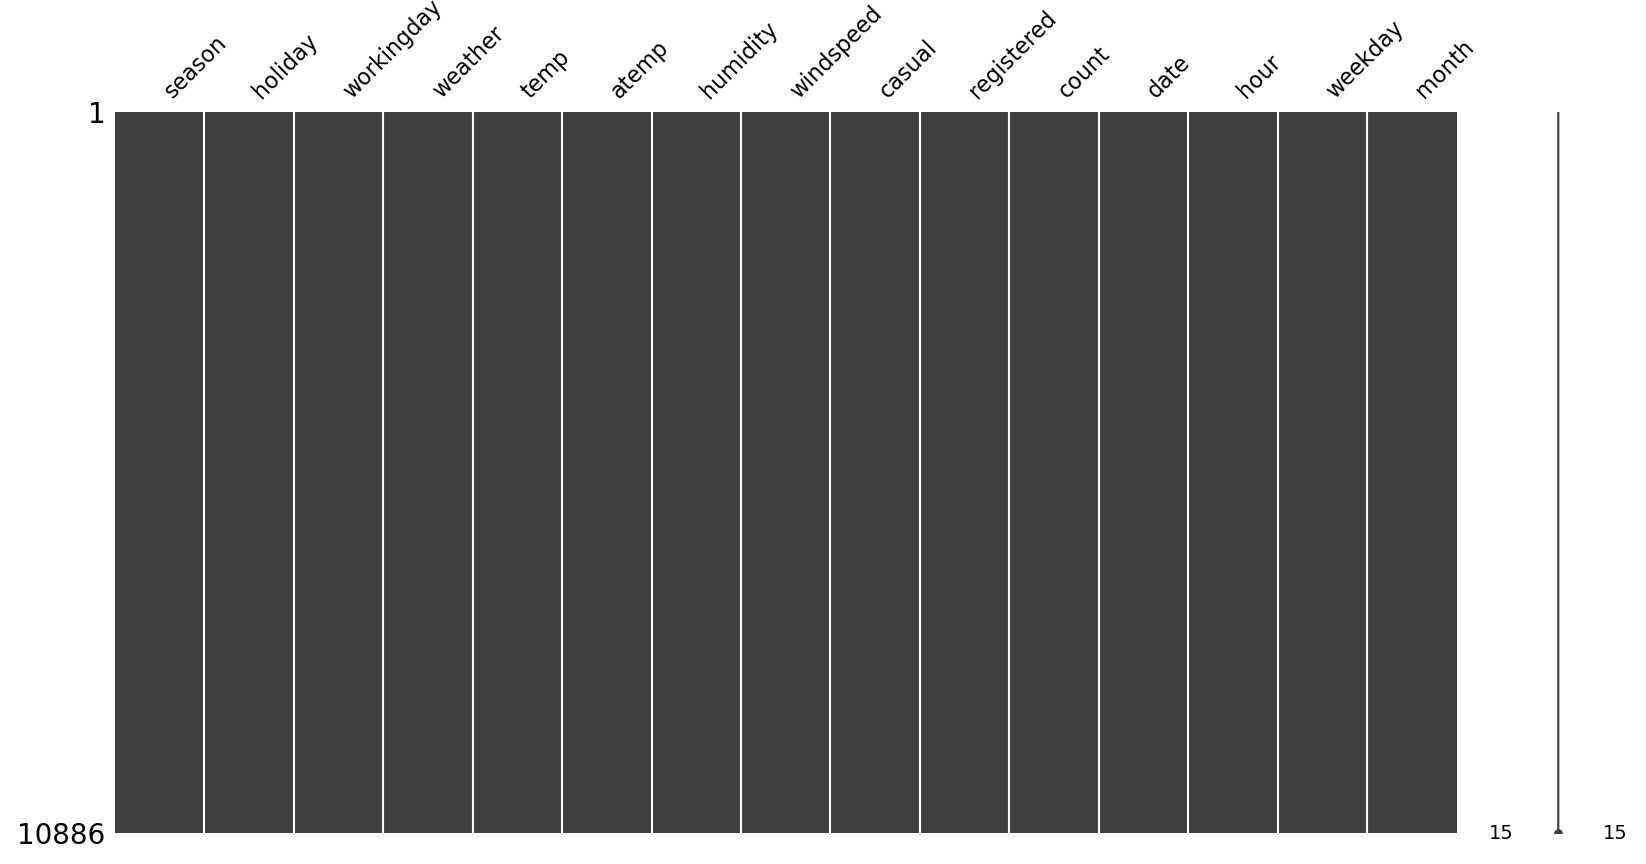
\includegraphics[scale=0.4]{./figure/Figure_1.eps}
	\caption{Missing values analysis}
\end{figure}
\end{slide}
%%
%%==========================================================================================	

%%==========================================================================================
%%
\begin{slide}{Outliers Analysis}
1:Spring season has got relatively lower count. \\
2:The boxplot with "Hour Of The Day" is quiet interesting.The median value are relatively higher at 7AM to 8AM and 5PM to 6PM.\\
3:Most of the outlier points are mainly contributed from "Working Day" than "Non Working Day". 
\begin{figure}[htbp]
	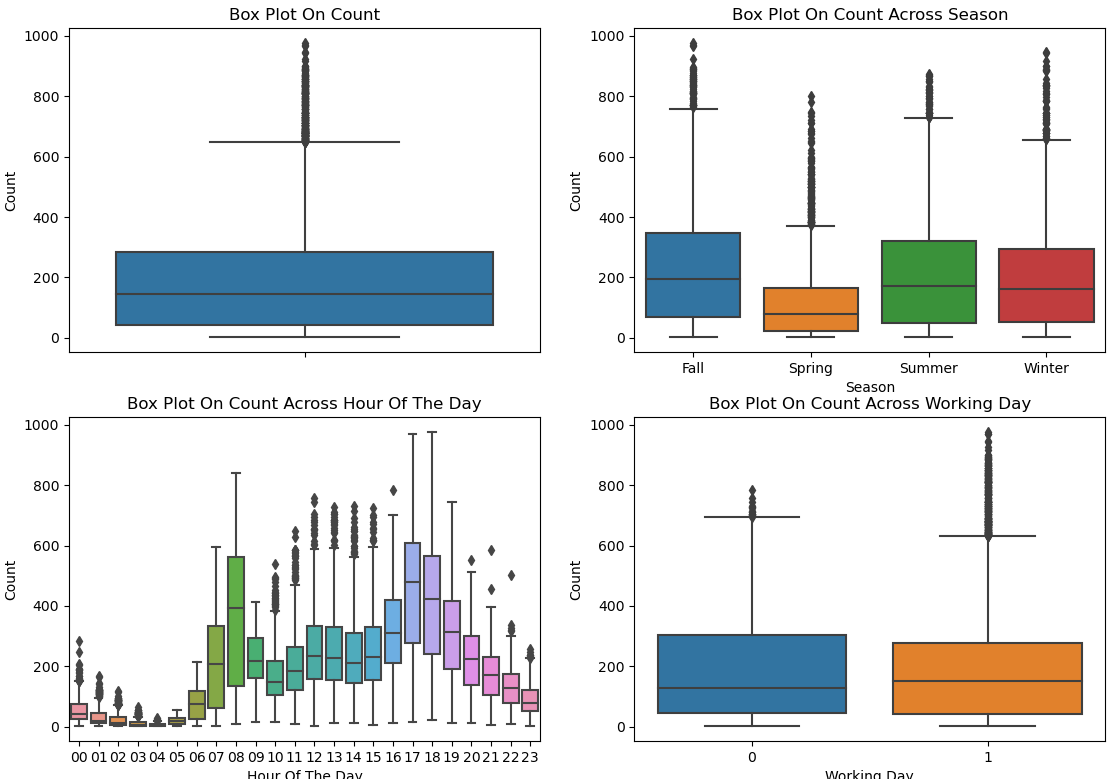
\includegraphics[scale=0.3]{./figure/Figure_2.eps}
	\caption{Missing values analysis}
\end{figure}
\end{slide}
%%
%%==========================================================================================	

%%==========================================================================================
%%
\begin{slide}{Correlation Analysis}
	1:temp and humidity features has got positive and negative correlation with count respectively. the count variable has got little dependency on "temp" and "humidity". \\
	2:"Casual" and "Registered" are also not taken into account since they are leakage variables in nature and need to dropped during model building. \\
	3:windspeed is not gonna be really useful numerical feature.
	\begin{figure}[htbp]
		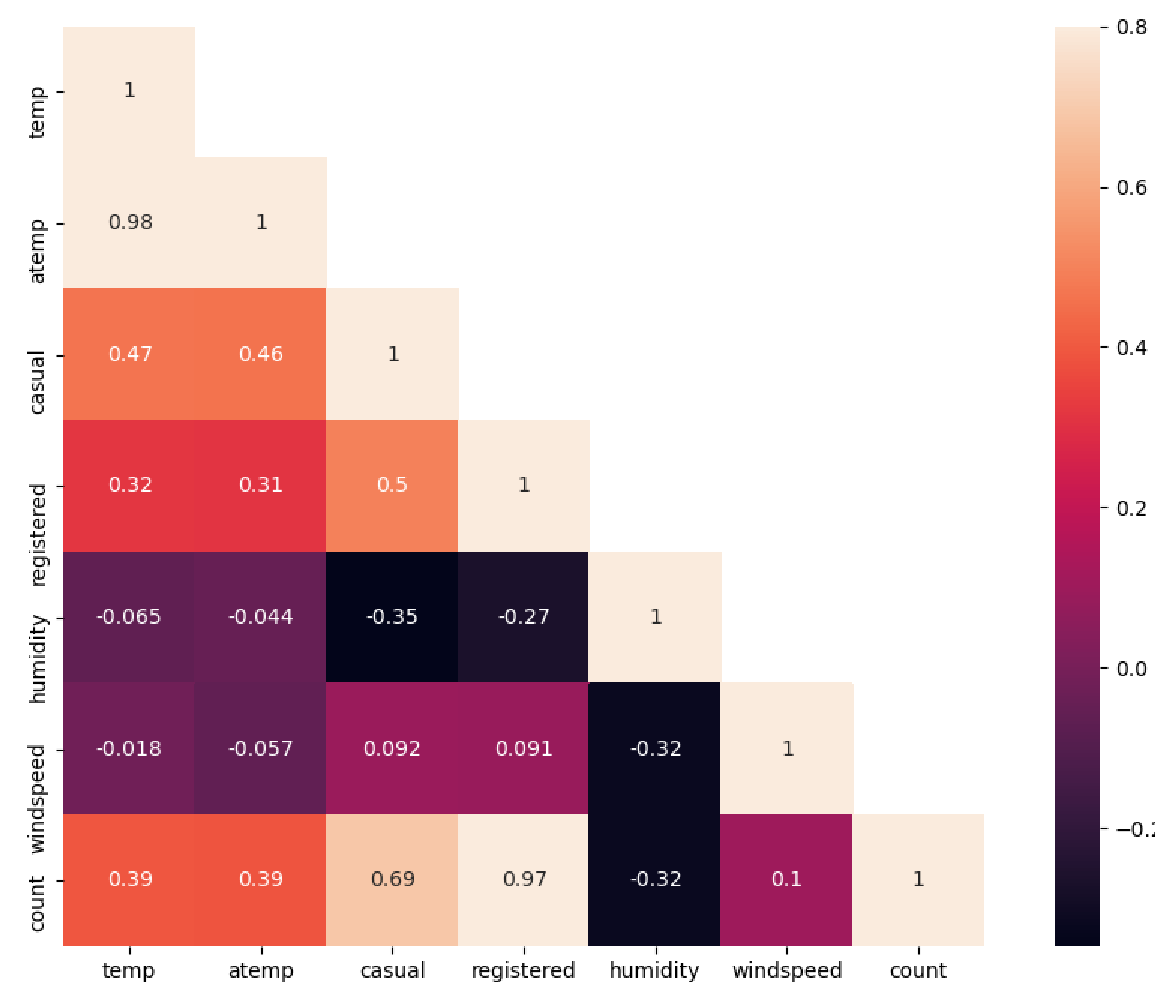
\includegraphics[scale=0.4]{./figure/Figure_3.eps}
		\caption{Correlation Analysis I}
	\end{figure}
\end{slide}
%%
%%==========================================================================================	

%%==========================================================================================
%%
\begin{slide}{}
	Regression plot in seaborn is one useful way to depict the relationship between two features. Here we consider "count" vs "temp", "humidity", "windspeed".
	\begin{figure}[htbp]
		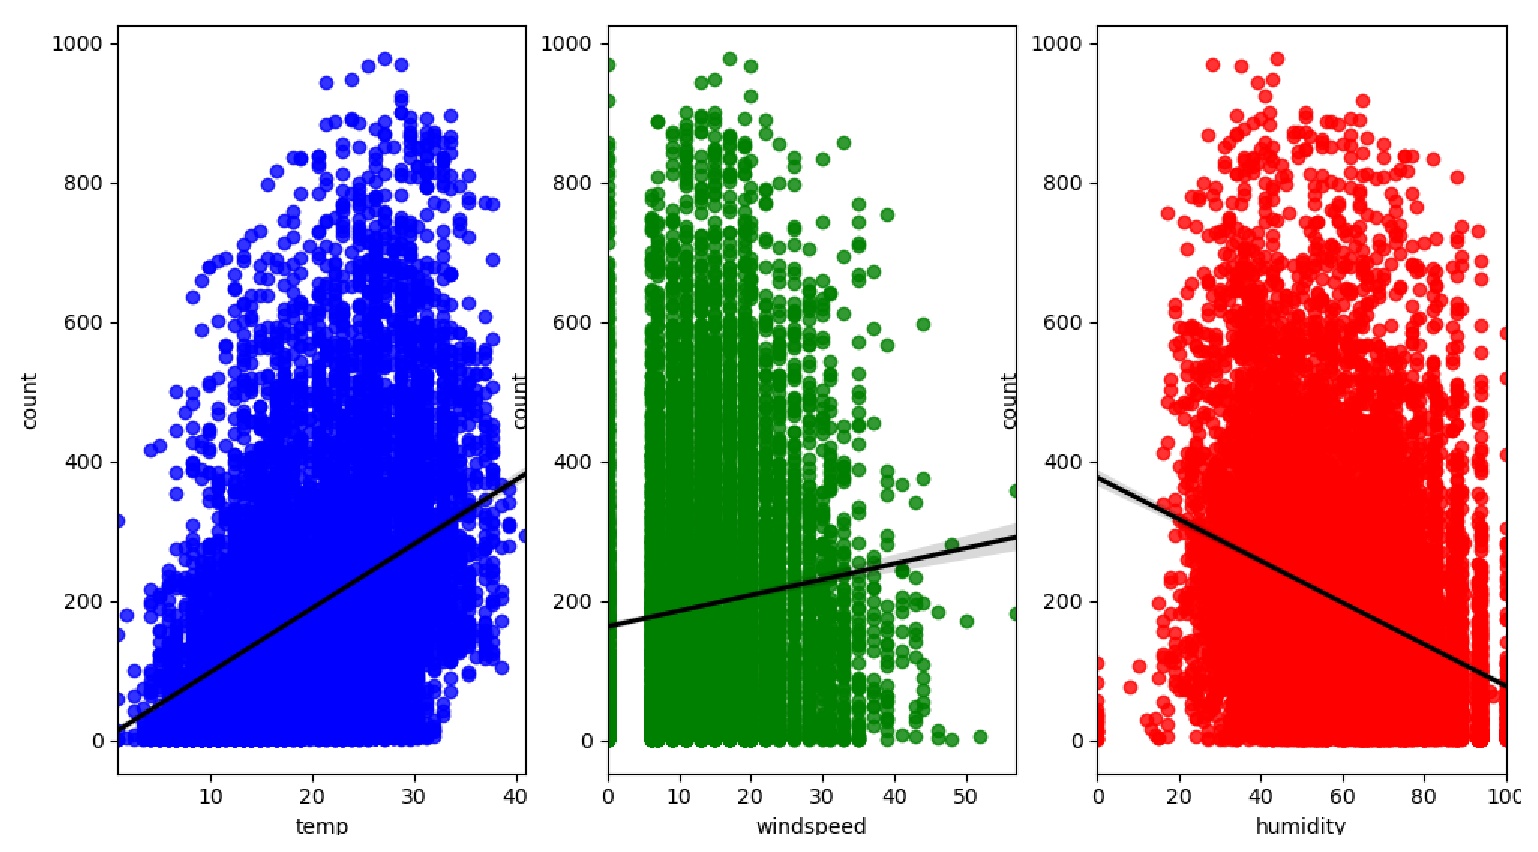
\includegraphics[scale=0.6]{./figure/Figure_4.eps}
		\caption{Correlation Analysis II}
	\end{figure}
\end{slide}
%%
%%==========================================================================================	

%%==========================================================================================
%%
\begin{slide}{Visualizing Distribution Of Data}
	 It is desirable to have Normal distribution as most of the machine learning techniques require dependent variable to be Normal. One possible solution is to take log transformation on "count" variable after removing outlier data points.
	\begin{figure}[htbp]
		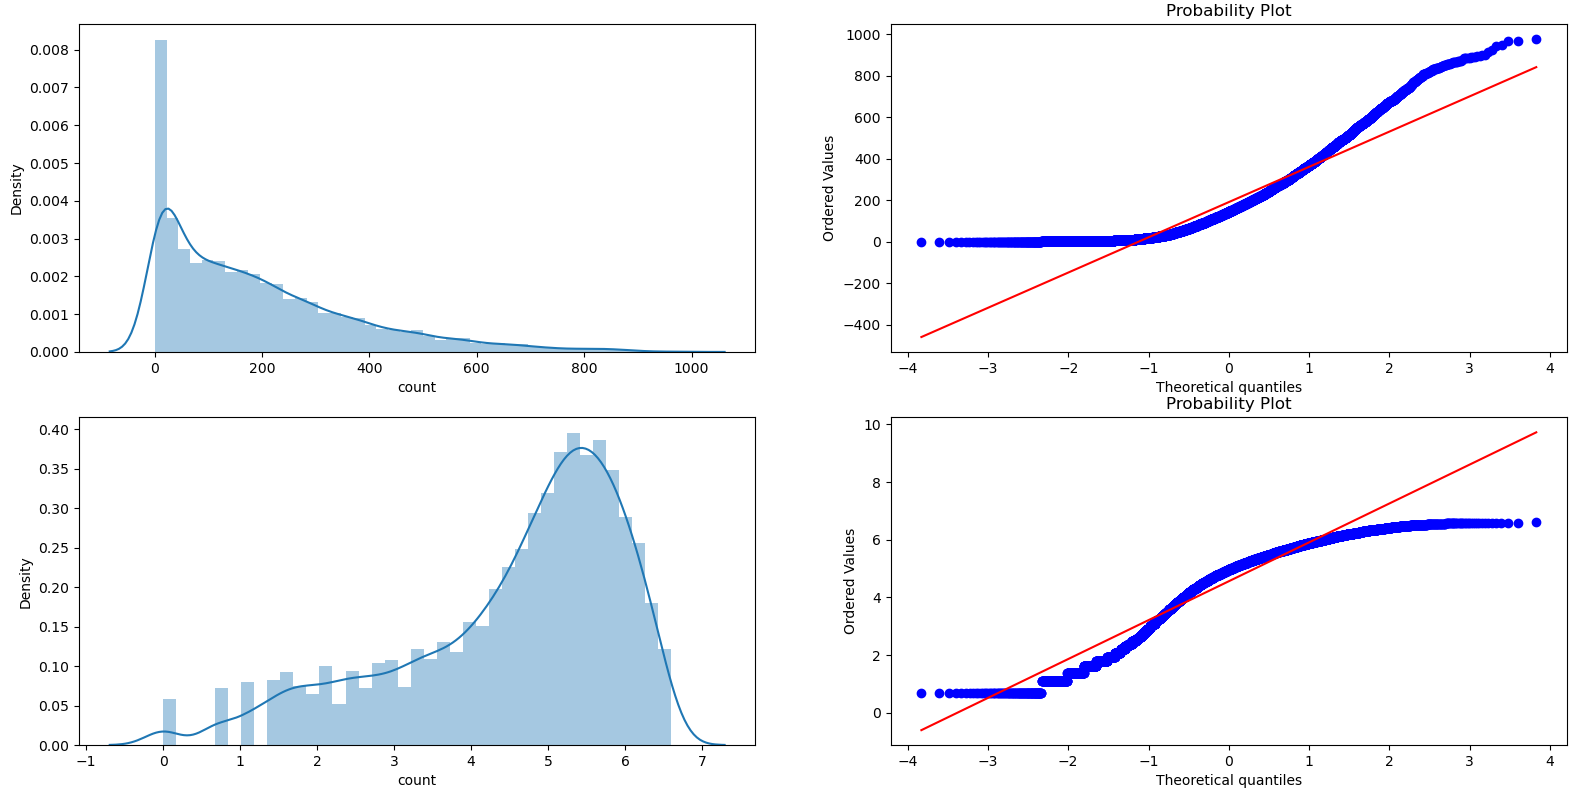
\includegraphics[scale=0.4]{./figure/Figure_5.eps}
		\caption{Visualizing Distribution Of Data}
	\end{figure}
\end{slide}
%%
%%==========================================================================================	

%%==========================================================================================
%%
\begin{slide}{Visualizing Count}
	1:It is quiet obvious that people tend to rent bike during summer season. Therefore June, July and August has got relatively higher demand for bicycle.\\
	2:On weekdays more people tend to rent bicycle around 7AM-8AM and 5PM-6PM. 
	\begin{figure}[htbp]
		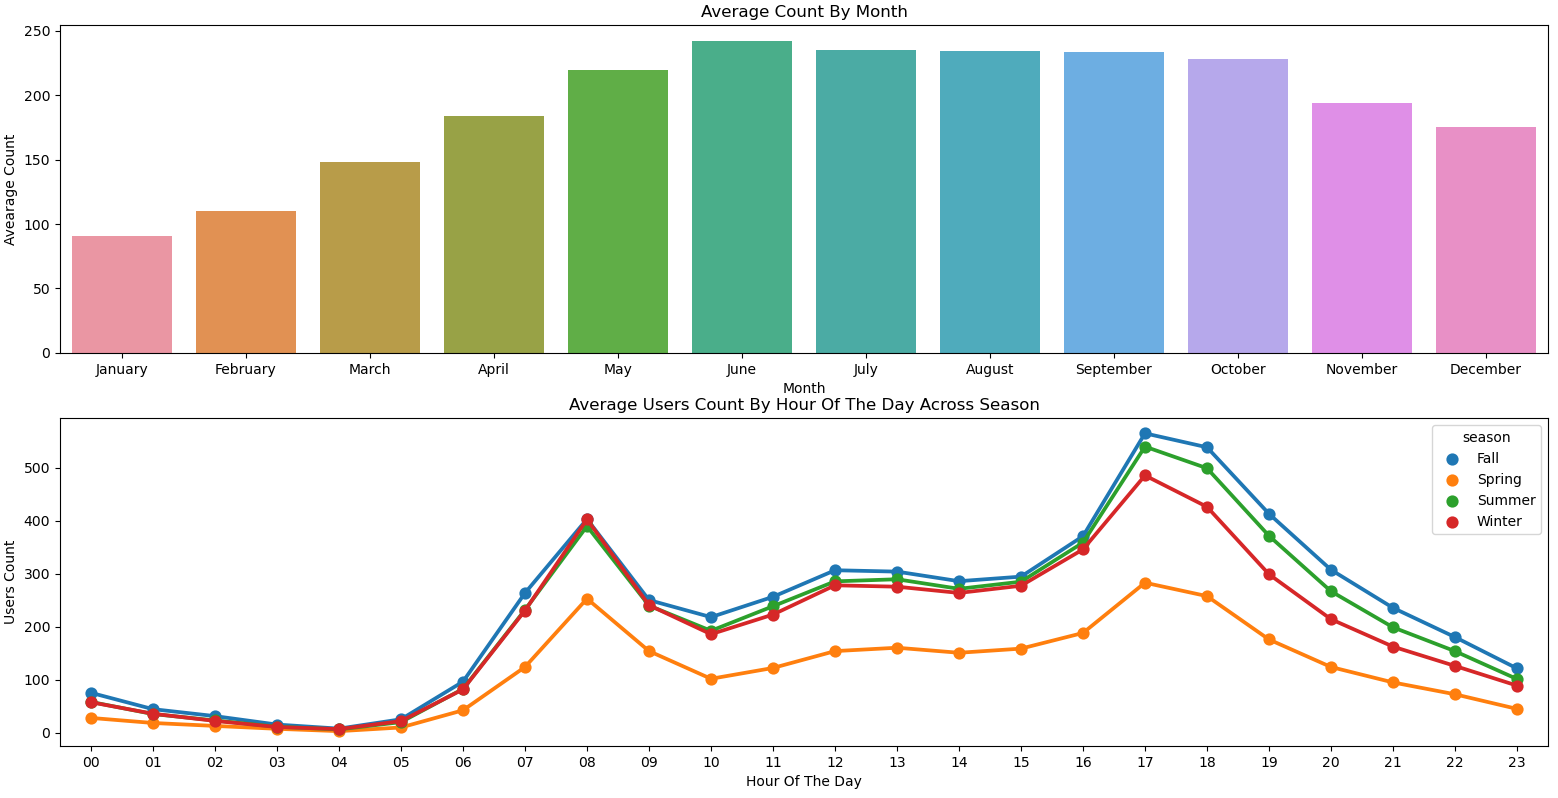
\includegraphics[scale=0.4]{./figure/Figure_6.eps}
		\caption{Visualizing Count I}
	\end{figure}
\end{slide}
%%
%%==========================================================================================	
%%==========================================================================================
%%
\begin{slide}{}
	1:On "Saturday" and "Sunday".More people tend to rent bicycle between 10AM and 4PM.\\
	2:Registered user contribute the peak around 7AM-8AM and 5PM-6PM.
	\begin{figure}[htbp]
		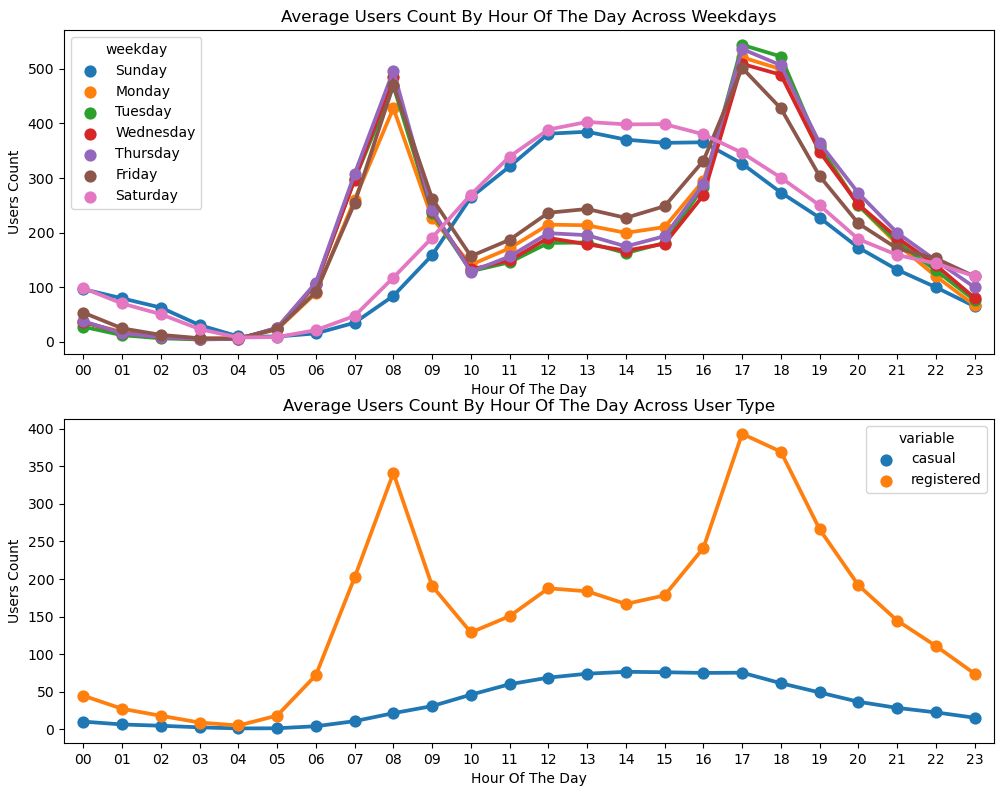
\includegraphics[scale=0.4]{./figure/Figure_7.eps}
		\caption{Visualizing Count II}
	\end{figure}
\end{slide}
%%
%%==========================================================================================

\section{Feature Engineering and Model}
%\begin{slide}{Algorithm one}
%\includegraphics*[scale=0.2]{1.png}
%\end{slide}
%%==========================================================================================
\begin{slide}[toc=,bm=]{Feature Processing}
	Split the given date into "date, hour, year, weekday, month".
	\begin{figure}[htbp]
		
\includegraphics[scale=0.8]{./figure/1.eps}
		\caption{Time feature processing}
	\end{figure}
	According to visual analysis, select features that have strong correlation with count.
	\begin{figure}[htbp]
		
\includegraphics[scale=0.75]{./figure/2.eps}
		\caption{Feature selection}
	\end{figure}
\end{slide}
%%
\begin{slide}[toc=,bm=]{Splitting train and test date}
	Divide train set and test set according to whether there is count attribute.
	\begin{figure}[htbp]
		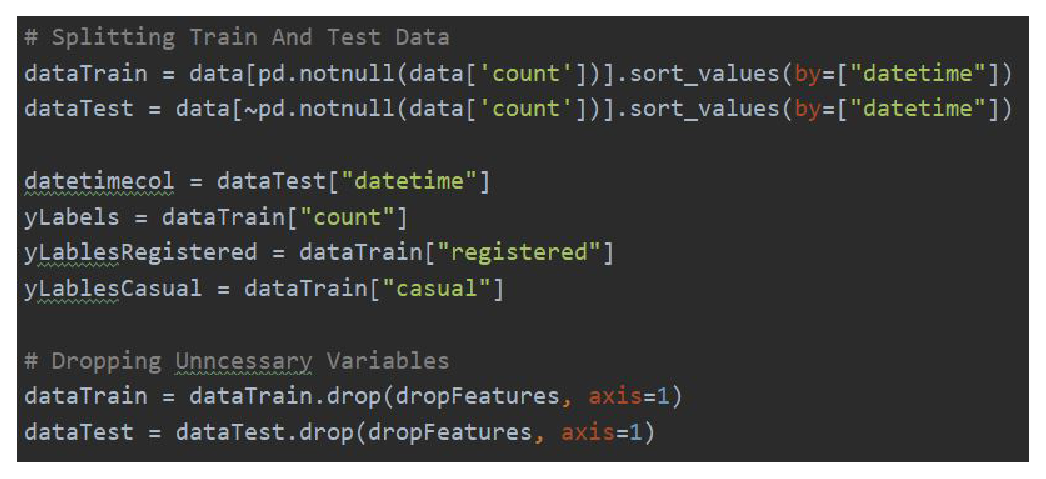
\includegraphics[scale=1]{./figure/3.eps}
		\caption{Training set and test set division}
	\end{figure}
\end{slide}
%%

\begin{slide}[toc=,bm=]{Model}
	I have choose the Ensemble Model - Gradient Boost. Compare the distribution of train and test results.It confirms visually that the model has not predicted really bad and not suffering from major overfitting problem.
	\begin{figure}[htbp]
	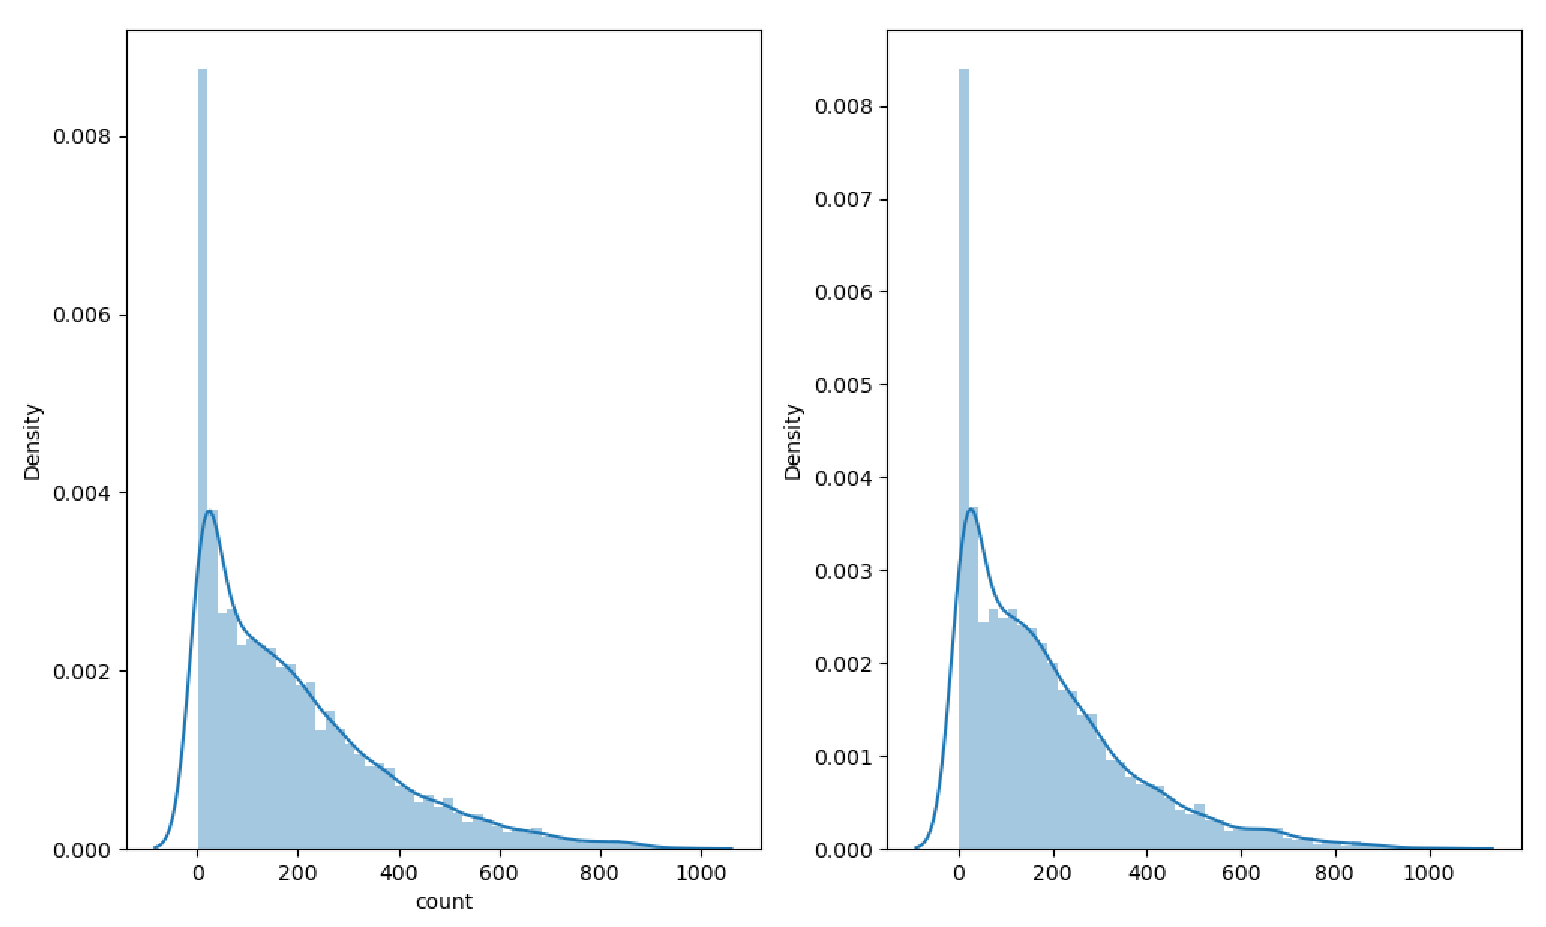
\includegraphics[scale=0.5]{./figure/models_Figure_1.eps}
	\caption{Distribution of train and test results}
	\end{figure}
\end{slide}

\section{Conclusion}
%%==========================================================================================
\begin{slide}[toc=,bm=]{Conclusion}
Using RMSLE to calculate the error, it penalizes under-prediction even more.\\
RMSLE Value For Gradient Boost:  0.189973542608\\
The score of my submission in kaggle is 0.41867. Ranked 428 among 3242 teams.\\
\begin{figure}[htbp]
	
\includegraphics[scale=0.8]{./figure/428-3242.eps}
	\caption{The score of my submission}
\end{figure}


\end{slide}
%%
%%==========================================================================================


%%==========================================================================================
% TODO: Contact Page
\begin{wideslide}[toc=,bm=]{Contact Information}
\centering
\vspace{\stretch{1}}
\twocolumn[
lcolwidth=0.35\linewidth,
rcolwidth=0.65\linewidth
]
{
% \centerline{
\includegraphics[scale=.2]{tulip-logo.eps}}
}
{
\vspace{\stretch{1}}
Bing Liu\\
College of Computer Science and Technology\\
Jilin University, China
\begin{description}
 \item[\textcolor{orange}{\faEnvelope}] \href{mailto:bliu@tulip.academy}
 {\textsc{\footnotesize{bliu@tulip.academy}}}

 \item[\textcolor{orange}{\faHome}] \href{http://www.tulip.org.au}
 {\textsc{\footnotesize{Team for Universal Learning and Intelligent Processing}}}
\end{description}
}
\vspace{\stretch{1}}
\end{wideslide}

\end{document}

\endinput
